\pgfdeclareplotmark{cross} {
\pgfpathmoveto{\pgfpoint{-0.3\pgfplotmarksize}{\pgfplotmarksize}}
\pgfpathlineto{\pgfpoint{+0.3\pgfplotmarksize}{\pgfplotmarksize}}
\pgfpathlineto{\pgfpoint{+0.3\pgfplotmarksize}{0.3\pgfplotmarksize}}
\pgfpathlineto{\pgfpoint{+1\pgfplotmarksize}{0.3\pgfplotmarksize}}
\pgfpathlineto{\pgfpoint{+1\pgfplotmarksize}{-0.3\pgfplotmarksize}}
\pgfpathlineto{\pgfpoint{+0.3\pgfplotmarksize}{-0.3\pgfplotmarksize}}
\pgfpathlineto{\pgfpoint{+0.3\pgfplotmarksize}{-1.\pgfplotmarksize}}
\pgfpathlineto{\pgfpoint{-0.3\pgfplotmarksize}{-1.\pgfplotmarksize}}
\pgfpathlineto{\pgfpoint{-0.3\pgfplotmarksize}{-0.3\pgfplotmarksize}}
\pgfpathlineto{\pgfpoint{-1.\pgfplotmarksize}{-0.3\pgfplotmarksize}}
\pgfpathlineto{\pgfpoint{-1.\pgfplotmarksize}{0.3\pgfplotmarksize}}
\pgfpathlineto{\pgfpoint{-0.3\pgfplotmarksize}{0.3\pgfplotmarksize}}
\pgfpathclose
\pgfusepathqstroke
}
\pgfdeclareplotmark{cross*} {
\pgfpathmoveto{\pgfpoint{-0.3\pgfplotmarksize}{\pgfplotmarksize}}
\pgfpathlineto{\pgfpoint{+0.3\pgfplotmarksize}{\pgfplotmarksize}}
\pgfpathlineto{\pgfpoint{+0.3\pgfplotmarksize}{0.3\pgfplotmarksize}}
\pgfpathlineto{\pgfpoint{+1\pgfplotmarksize}{0.3\pgfplotmarksize}}
\pgfpathlineto{\pgfpoint{+1\pgfplotmarksize}{-0.3\pgfplotmarksize}}
\pgfpathlineto{\pgfpoint{+0.3\pgfplotmarksize}{-0.3\pgfplotmarksize}}
\pgfpathlineto{\pgfpoint{+0.3\pgfplotmarksize}{-1.\pgfplotmarksize}}
\pgfpathlineto{\pgfpoint{-0.3\pgfplotmarksize}{-1.\pgfplotmarksize}}
\pgfpathlineto{\pgfpoint{-0.3\pgfplotmarksize}{-0.3\pgfplotmarksize}}
\pgfpathlineto{\pgfpoint{-1.\pgfplotmarksize}{-0.3\pgfplotmarksize}}
\pgfpathlineto{\pgfpoint{-1.\pgfplotmarksize}{0.3\pgfplotmarksize}}
\pgfpathlineto{\pgfpoint{-0.3\pgfplotmarksize}{0.3\pgfplotmarksize}}
\pgfpathclose
\pgfusepathqfillstroke
}
\pgfdeclareplotmark{newstar} {
\pgfpathmoveto{\pgfqpoint{0pt}{\pgfplotmarksize}}
\pgfpathlineto{\pgfqpointpolar{44}{0.5\pgfplotmarksize}}
\pgfpathlineto{\pgfqpointpolar{18}{\pgfplotmarksize}}
\pgfpathlineto{\pgfqpointpolar{-20}{0.5\pgfplotmarksize}}
\pgfpathlineto{\pgfqpointpolar{-54}{\pgfplotmarksize}}
\pgfpathlineto{\pgfqpointpolar{-90}{0.5\pgfplotmarksize}}
\pgfpathlineto{\pgfqpointpolar{234}{\pgfplotmarksize}}
\pgfpathlineto{\pgfqpointpolar{198}{0.5\pgfplotmarksize}}
\pgfpathlineto{\pgfqpointpolar{162}{\pgfplotmarksize}}
\pgfpathlineto{\pgfqpointpolar{134}{0.5\pgfplotmarksize}}
\pgfpathclose
\pgfusepathqstroke
}
\pgfdeclareplotmark{newstar*} {
\pgfpathmoveto{\pgfqpoint{0pt}{\pgfplotmarksize}}
\pgfpathlineto{\pgfqpointpolar{44}{0.5\pgfplotmarksize}}
\pgfpathlineto{\pgfqpointpolar{18}{\pgfplotmarksize}}
\pgfpathlineto{\pgfqpointpolar{-20}{0.5\pgfplotmarksize}}
\pgfpathlineto{\pgfqpointpolar{-54}{\pgfplotmarksize}}
\pgfpathlineto{\pgfqpointpolar{-90}{0.5\pgfplotmarksize}}
\pgfpathlineto{\pgfqpointpolar{234}{\pgfplotmarksize}}
\pgfpathlineto{\pgfqpointpolar{198}{0.5\pgfplotmarksize}}
\pgfpathlineto{\pgfqpointpolar{162}{\pgfplotmarksize}}
\pgfpathlineto{\pgfqpointpolar{134}{0.5\pgfplotmarksize}}
\pgfpathclose
\pgfusepathqfillstroke
}
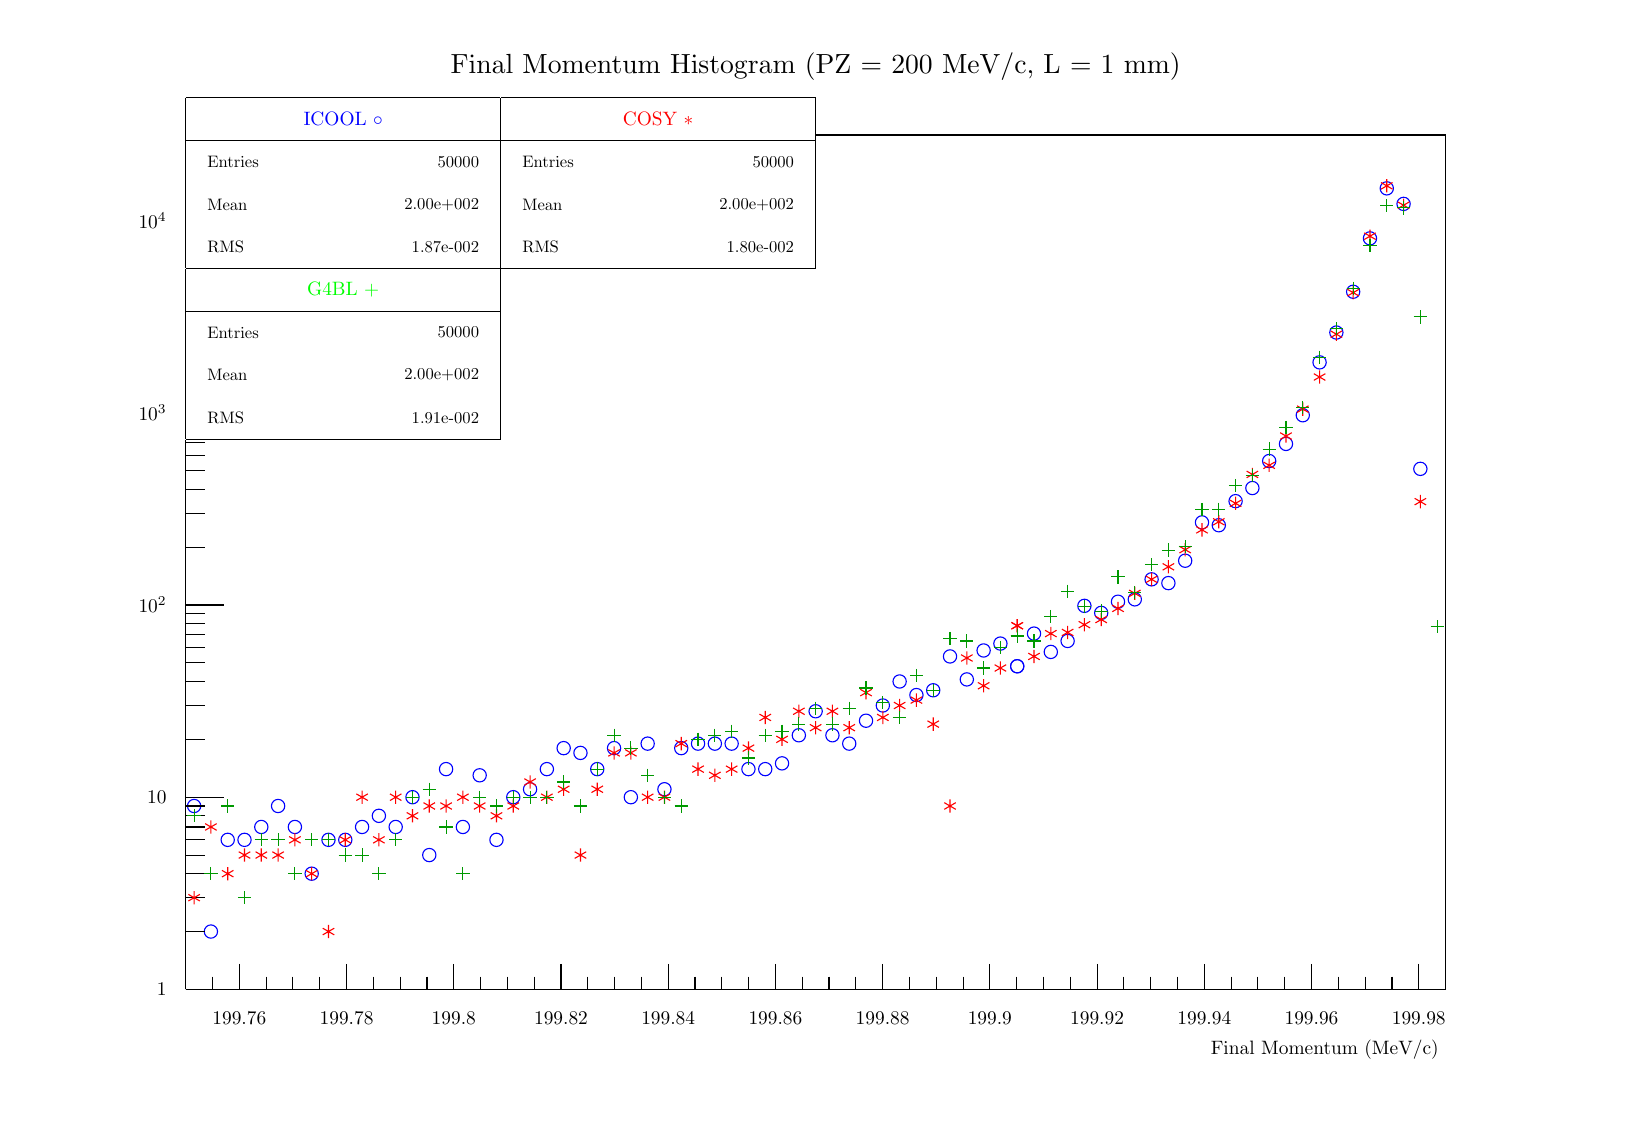
\begin{tikzpicture}
\definecolor{c}{rgb}{1,1,1};
\draw [color=c, fill=c] (0,0) rectangle (20,13.5632);
\draw [color=c, fill=c] (2,1.35632) rectangle (18,12.2069);
\definecolor{c}{rgb}{0,0,0};
\draw [c] (2,1.35632) -- (2,12.2069) -- (18,12.2069) -- (18,1.35632) -- (2,1.35632);
\definecolor{c}{rgb}{1,1,1};
\draw [color=c, fill=c] (2,1.35632) rectangle (18,12.2069);
\definecolor{c}{rgb}{0,0,0};
\draw [c] (2,1.35632) -- (2,12.2069) -- (18,12.2069) -- (18,1.35632) -- (2,1.35632);
\definecolor{c}{rgb}{0,0,1};
\foreach \P in
 {(2.10667,3.68552),(2.32,2.0911),(2.53333,3.2557),(2.74667,3.2557),(2.96,3.41911),(3.17333,3.68552),(3.38667,3.41911),(3.6,2.82588),(3.81333,3.2557),(4.02667,3.2557),(4.24,3.41911),(4.45333,3.56066),(4.66667,3.41911),(4.88,3.79721),(5.09333,3.06243)
,(5.30667,4.15389),(5.52,3.41911),(5.73333,4.07533),(5.94667,3.2557),(6.16,3.79721),(6.37333,3.89824),(6.58667,4.15389),(6.8,4.4203),(7.01333,4.35971),(7.22667,4.15389),(7.44,4.4203),(7.65333,3.79721),(7.86667,4.47762),(8.08,3.89824),(8.29333,4.4203)
,(8.50667,4.47762),(8.72,4.47762),(8.93333,4.47762),(9.14667,4.15389),(9.36,4.15389),(9.57333,4.22703),(9.78667,4.58371),(10,4.88867),(10.2133,4.58371),(10.4267,4.47762),(10.64,4.76854),(10.8533,4.96181),(11.0667,5.26677),(11.28,5.09449),(11.4933,5.1
5508),(11.7067,5.5849),(11.92,5.29295),(12.1333,5.66065),(12.3467,5.74831),(12.56,5.46004)}{\draw[mark options={color=c,fill=c},mark size=2.402402pt,mark=o] plot coordinates {\P};}
\foreach \P in
 {(12.56,5.46004),(12.7733,5.87504),(12.9867,5.64222),(13.2,5.78144),(13.4133,6.22744),(13.6267,6.13812),(13.84,6.27967),(14.0533,6.30982),(14.2667,6.56405),(14.48,6.51622),(14.6933,6.8006),(14.9067,7.28708),(15.12,7.251),(15.3333,7.55698),(15.5467,7
.72344),(15.76,8.06623),(15.9733,8.2841),(16.1867,8.64779),(16.4,9.3196),(16.6133,9.69839),(16.8267,10.2163),(17.04,10.8941),(17.2533,11.5294),(17.4667,11.3321),(17.68,7.96727)}{\draw[mark options={color=c,fill=c},mark size=2.402402pt,mark=o] plot
 coordinates {\P};}
\definecolor{c}{rgb}{1,1,1};
\draw [color=c, fill=c] (2,10.5115) rectangle (6,12.6816);
\definecolor{c}{rgb}{0,0,0};
\draw [c] (2,10.5115) -- (6,10.5115);
\draw [c] (6,10.5115) -- (6,12.6816);
\draw [c] (6,12.6816) -- (2,12.6816);
\draw [c] (2,12.6816) -- (2,10.5115);
\draw[color=blue](4,12.4103) node[scale=0.7, rotate=0]{ICOOL $\circ$};
\draw [c] (2,12.1391) -- (6,12.1391);
\draw [anchor= west] (2.2,11.8678) node[scale=0.6, rotate=0]{Entries };
\draw [anchor= east] (5.8,11.8678) node[scale=0.6, rotate=0]{ 50000};
\draw [anchor= west] (2.2,11.3253) node[scale=0.6, rotate=0]{Mean  };
\draw [anchor= east] (5.8,11.3253) node[scale=0.6, rotate=0]{ 2.00e+002};
\draw [anchor= west] (2.2,10.7828) node[scale=0.6, rotate=0]{RMS   };
\draw [anchor= east] (5.8,10.7828) node[scale=0.6, rotate=0]{ 1.87e-002};
\draw [c] (2,1.35632) -- (18,1.35632);
\draw [anchor= east] (18,0.596782) node[scale=0.7, rotate=0]{Final Momentum (MeV/c)};
\draw [c] (2.68085,1.68184) -- (2.68085,1.35632);
\draw [c] (3.02128,1.51908) -- (3.02128,1.35632);
\draw [c] (3.3617,1.51908) -- (3.3617,1.35632);
\draw [c] (3.70213,1.51908) -- (3.70213,1.35632);
\draw [c] (4.04255,1.68184) -- (4.04255,1.35632);
\draw [c] (4.38298,1.51908) -- (4.38298,1.35632);
\draw [c] (4.7234,1.51908) -- (4.7234,1.35632);
\draw [c] (5.06383,1.51908) -- (5.06383,1.35632);
\draw [c] (5.40426,1.68184) -- (5.40426,1.35632);
\draw [c] (5.74468,1.51908) -- (5.74468,1.35632);
\draw [c] (6.08511,1.51908) -- (6.08511,1.35632);
\draw [c] (6.42553,1.51908) -- (6.42553,1.35632);
\draw [c] (6.76596,1.68184) -- (6.76596,1.35632);
\draw [c] (7.10638,1.51908) -- (7.10638,1.35632);
\draw [c] (7.44681,1.51908) -- (7.44681,1.35632);
\draw [c] (7.78723,1.51908) -- (7.78723,1.35632);
\draw [c] (8.12766,1.68184) -- (8.12766,1.35632);
\draw [c] (8.46809,1.51908) -- (8.46809,1.35632);
\draw [c] (8.80851,1.51908) -- (8.80851,1.35632);
\draw [c] (9.14894,1.51908) -- (9.14894,1.35632);
\draw [c] (9.48936,1.68184) -- (9.48936,1.35632);
\draw [c] (9.82979,1.51908) -- (9.82979,1.35632);
\draw [c] (10.1702,1.51908) -- (10.1702,1.35632);
\draw [c] (10.5106,1.51908) -- (10.5106,1.35632);
\draw [c] (10.8511,1.68184) -- (10.8511,1.35632);
\draw [c] (11.1915,1.51908) -- (11.1915,1.35632);
\draw [c] (11.5319,1.51908) -- (11.5319,1.35632);
\draw [c] (11.8723,1.51908) -- (11.8723,1.35632);
\draw [c] (12.2128,1.68184) -- (12.2128,1.35632);
\draw [c] (12.5532,1.51908) -- (12.5532,1.35632);
\draw [c] (12.8936,1.51908) -- (12.8936,1.35632);
\draw [c] (13.234,1.51908) -- (13.234,1.35632);
\draw [c] (13.5745,1.68184) -- (13.5745,1.35632);
\draw [c] (13.9149,1.51908) -- (13.9149,1.35632);
\draw [c] (14.2553,1.51908) -- (14.2553,1.35632);
\draw [c] (14.5957,1.51908) -- (14.5957,1.35632);
\draw [c] (14.9362,1.68184) -- (14.9362,1.35632);
\draw [c] (15.2766,1.51908) -- (15.2766,1.35632);
\draw [c] (15.617,1.51908) -- (15.617,1.35632);
\draw [c] (15.9574,1.51908) -- (15.9574,1.35632);
\draw [c] (16.2979,1.68184) -- (16.2979,1.35632);
\draw [c] (16.6383,1.51908) -- (16.6383,1.35632);
\draw [c] (16.9787,1.51908) -- (16.9787,1.35632);
\draw [c] (17.3191,1.51908) -- (17.3191,1.35632);
\draw [c] (17.6596,1.68184) -- (17.6596,1.35632);
\draw [c] (2.68085,1.68184) -- (2.68085,1.35632);
\draw [c] (2.34043,1.51908) -- (2.34043,1.35632);
\draw [c] (2,1.51908) -- (2,1.35632);
\draw [c] (17.6596,1.68184) -- (17.6596,1.35632);
\draw [c] (18,1.51908) -- (18,1.35632);
\draw [anchor=base] (2.68085,0.908736) node[scale=0.7, rotate=0]{199.76};
\draw [anchor=base] (4.04255,0.908736) node[scale=0.7, rotate=0]{199.78};
\draw [anchor=base] (5.40426,0.908736) node[scale=0.7, rotate=0]{199.8};
\draw [anchor=base] (6.76596,0.908736) node[scale=0.7, rotate=0]{199.82};
\draw [anchor=base] (8.12766,0.908736) node[scale=0.7, rotate=0]{199.84};
\draw [anchor=base] (9.48936,0.908736) node[scale=0.7, rotate=0]{199.86};
\draw [anchor=base] (10.8511,0.908736) node[scale=0.7, rotate=0]{199.88};
\draw [anchor=base] (12.2128,0.908736) node[scale=0.7, rotate=0]{199.9};
\draw [anchor=base] (13.5745,0.908736) node[scale=0.7, rotate=0]{199.92};
\draw [anchor=base] (14.9362,0.908736) node[scale=0.7, rotate=0]{199.94};
\draw [anchor=base] (16.2979,0.908736) node[scale=0.7, rotate=0]{199.96};
\draw [anchor=base] (17.6596,0.908736) node[scale=0.7, rotate=0]{199.98};
\draw [c] (2,1.35632) -- (2,12.2069);
\draw [c] (2.48,1.35632) -- (2,1.35632);
\draw [anchor= east] (1.844,1.35632) node[scale=0.7, rotate=0]{1};
\draw [c] (2.24,2.0911) -- (2,2.0911);
\draw [c] (2.24,2.52092) -- (2,2.52092);
\draw [c] (2.24,2.82589) -- (2,2.82589);
\draw [c] (2.24,3.06243) -- (2,3.06243);
\draw [c] (2.24,3.2557) -- (2,3.2557);
\draw [c] (2.24,3.41911) -- (2,3.41911);
\draw [c] (2.24,3.56067) -- (2,3.56067);
\draw [c] (2.24,3.68552) -- (2,3.68552);
\draw [c] (2.48,3.79721) -- (2,3.79721);
\draw [anchor= east] (1.844,3.79721) node[scale=0.7, rotate=0]{10};
\draw [c] (2.24,4.53199) -- (2,4.53199);
\draw [c] (2.24,4.96181) -- (2,4.96181);
\draw [c] (2.24,5.26677) -- (2,5.26677);
\draw [c] (2.24,5.50332) -- (2,5.50332);
\draw [c] (2.24,5.69659) -- (2,5.69659);
\draw [c] (2.24,5.86) -- (2,5.86);
\draw [c] (2.24,6.00155) -- (2,6.00155);
\draw [c] (2.24,6.12641) -- (2,6.12641);
\draw [c] (2.48,6.2381) -- (2,6.2381);
\draw [anchor= east] (1.844,6.2381) node[scale=0.7, rotate=0]{$10^{2}$};
\draw [c] (2.24,6.97288) -- (2,6.97288);
\draw [c] (2.24,7.4027) -- (2,7.4027);
\draw [c] (2.24,7.70766) -- (2,7.70766);
\draw [c] (2.24,7.94421) -- (2,7.94421);
\draw [c] (2.24,8.13748) -- (2,8.13748);
\draw [c] (2.24,8.30089) -- (2,8.30089);
\draw [c] (2.24,8.44244) -- (2,8.44244);
\draw [c] (2.24,8.5673) -- (2,8.5673);
\draw [c] (2.48,8.67899) -- (2,8.67899);
\draw [anchor= east] (1.844,8.67899) node[scale=0.7, rotate=0]{$10^{3}$};
\draw [c] (2.24,9.41377) -- (2,9.41377);
\draw [c] (2.24,9.84359) -- (2,9.84359);
\draw [c] (2.24,10.1485) -- (2,10.1485);
\draw [c] (2.24,10.3851) -- (2,10.3851);
\draw [c] (2.24,10.5784) -- (2,10.5784);
\draw [c] (2.24,10.7418) -- (2,10.7418);
\draw [c] (2.24,10.8833) -- (2,10.8833);
\draw [c] (2.24,11.0082) -- (2,11.0082);
\draw [c] (2.48,11.1199) -- (2,11.1199);
\draw [anchor= east] (1.844,11.1199) node[scale=0.7, rotate=0]{$10^{4}$};
\draw [c] (2.24,11.8547) -- (2,11.8547);
\definecolor{c}{rgb}{1,1,1};
\draw [color=c, fill=c] (2,10.5115) rectangle (6,12.6816);
\definecolor{c}{rgb}{0,0,0};
\draw [c] (2,10.5115) -- (6,10.5115);
\draw [c] (6,10.5115) -- (6,12.6816);
\draw [c] (6,12.6816) -- (2,12.6816);
\draw [c] (2,12.6816) -- (2,10.5115);
\draw[color=blue](4,12.4103) node[scale=0.7, rotate=0]{ICOOL $\circ$};
\draw [c] (2,12.1391) -- (6,12.1391);
\draw [anchor= west] (2.2,11.8678) node[scale=0.6, rotate=0]{Entries };
\draw [anchor= east] (5.8,11.8678) node[scale=0.6, rotate=0]{ 50000};
\draw [anchor= west] (2.2,11.3253) node[scale=0.6, rotate=0]{Mean  };
\draw [anchor= east] (5.8,11.3253) node[scale=0.6, rotate=0]{ 2.00e+002};
\draw [anchor= west] (2.2,10.7828) node[scale=0.6, rotate=0]{RMS   };
\draw [anchor= east] (5.8,10.7828) node[scale=0.6, rotate=0]{ 1.87e-002};
\draw (10,13.0816) node[scale=1, rotate=0]{Final Momentum Histogram (PZ = 200 MeV/c, L = 1 mm)};
\definecolor{c}{rgb}{1,0,0};
\foreach \P in
 {(2.10667,2.52092),(2.32,3.41911),(2.53333,2.82588),(2.74667,3.06243),(2.96,3.06243),(3.17333,3.06243),(3.38667,3.2557),(3.6,2.82588),(3.81333,2.0911),(4.02667,3.2557),(4.24,3.79721),(4.45333,3.2557),(4.66667,3.79721),(4.88,3.56066),(5.09333,3.68552
),(5.30667,3.68552),(5.52,3.79721),(5.73333,3.68552),(5.94667,3.56066),(6.16,3.68552),(6.37333,3.99048),(6.58667,3.79721),(6.8,3.89824),(7.01333,3.06243),(7.22667,3.89824),(7.44,4.35971),(7.65333,4.35971),(7.86667,3.79721),(8.08,3.79721),(8.29333,4.4
7762),(8.50667,4.15389),(8.72,4.07533),(8.93333,4.15389),(9.14667,4.4203),(9.36,4.81011),(9.57333,4.53199),(9.78667,4.88867),(10,4.68015),(10.2133,4.88867),(10.4267,4.68015),(10.64,5.12522),(10.8533,4.81011),(11.0667,4.96181),(11.28,5.03022),(11.4933
,4.72526),(11.7067,3.68552),(11.92,5.56509),(12.1333,5.2124),(12.3467,5.43773),(12.56,5.97471)}{\draw[mark options={color=c,fill=c},mark size=2.402402pt,mark=asterisk] plot coordinates {\P};}
\foreach \P in
 {(12.56,5.97471),(12.7733,5.5849),(12.9867,5.87504),(13.2,5.88986),(13.4133,5.98822),(13.6267,6.05327),(13.84,6.19482),(14.0533,6.38625),(14.2667,6.56405),(14.48,6.723),(14.6933,6.94059),(14.9067,7.19233),(15.12,7.29493),(15.3333,7.52912),(15.5467,7
.89651),(15.76,8.01196),(15.9733,8.38387),(16.1867,8.72565),(16.4,9.13326),(16.6133,9.67711),(16.8267,10.2051),(17.04,10.922),(17.2533,11.5614),(17.4667,11.3151),(17.68,7.55085)}{\draw[mark options={color=c,fill=c},mark size=2.402402pt,mark=asterisk]
 plot coordinates {\P};}
\definecolor{c}{rgb}{1,1,1};
\draw [color=c, fill=c] (6,10.5115) rectangle (10,12.6816);
\definecolor{c}{rgb}{0,0,0};
\draw [c] (6,10.5115) -- (10,10.5115);
\draw [c] (10,10.5115) -- (10,12.6816);
\draw [c] (10,12.6816) -- (6,12.6816);
\draw [c] (6,12.6816) -- (6,10.5115);
\draw [color=red](8,12.4103) node[scale=0.7, rotate=0]{COSY $*$};
\draw [c] (6,12.1391) -- (10,12.1391);
\draw [anchor= west] (6.2,11.8678) node[scale=0.6, rotate=0]{Entries };
\draw [anchor= east] (9.8,11.8678) node[scale=0.6, rotate=0]{ 50000};
\draw [anchor= west] (6.2,11.3253) node[scale=0.6, rotate=0]{Mean  };
\draw [anchor= east] (9.8,11.3253) node[scale=0.6, rotate=0]{ 2.00e+002};
\draw [anchor= west] (6.2,10.7828) node[scale=0.6, rotate=0]{RMS   };
\draw [anchor= east] (9.8,10.7828) node[scale=0.6, rotate=0]{ 1.80e-002};
\definecolor{c}{rgb}{1,1,1};
\draw [color=c, fill=c] (6,10.5115) rectangle (10,12.6816);
\definecolor{c}{rgb}{0,0,0};
\draw [c] (6,10.5115) -- (10,10.5115);
\draw [c] (10,10.5115) -- (10,12.6816);
\draw [c] (10,12.6816) -- (6,12.6816);
\draw [c] (6,12.6816) -- (6,10.5115);
\draw [color=red](8,12.4103) node[scale=0.7, rotate=0]{COSY $*$};
\draw [c] (6,12.1391) -- (10,12.1391);
\draw [anchor= west] (6.2,11.8678) node[scale=0.6, rotate=0]{Entries };
\draw [anchor= east] (9.8,11.8678) node[scale=0.6, rotate=0]{ 50000};
\draw [anchor= west] (6.2,11.3253) node[scale=0.6, rotate=0]{Mean  };
\draw [anchor= east] (9.8,11.3253) node[scale=0.6, rotate=0]{ 2.00e+002};
\draw [anchor= west] (6.2,10.7828) node[scale=0.6, rotate=0]{RMS   };
\draw [anchor= east] (9.8,10.7828) node[scale=0.6, rotate=0]{ 1.80e-002};
\definecolor{c}{rgb}{0,0.6,0};
\foreach \P in
 {(2.10667,3.56066),(2.32,2.82588),(2.53333,3.68552),(2.74667,2.52092),(2.96,3.2557),(3.17333,3.2557),(3.38667,2.82588),(3.6,3.2557),(3.81333,3.2557),(4.02667,3.06243),(4.24,3.06243),(4.45333,2.82588),(4.66667,3.2557),(4.88,3.79721),(5.09333,3.89824)
,(5.30667,3.41911),(5.52,2.82588),(5.73333,3.79721),(5.94667,3.68552),(6.16,3.79721),(6.37333,3.79721),(6.58667,3.79721),(6.8,3.99048),(7.01333,3.68552),(7.22667,4.15389),(7.44,4.58371),(7.65333,4.4203),(7.86667,4.07533),(8.08,3.79721),(8.29333,3.685
52),(8.50667,4.53199),(8.72,4.58371),(8.93333,4.63303),(9.14667,4.29544),(9.36,4.58371),(9.57333,4.63303),(9.78667,4.72526),(10,4.92587),(10.2133,4.72526),(10.4267,4.92587),(10.64,5.18413),(10.8533,4.99657),(11.0667,4.81011),(11.28,5.34344),(11.4933,
5.15508),(11.7067,5.81357),(11.92,5.78144),(12.1333,5.43773),(12.3467,5.69659),(12.56,5.84475)}{\draw[mark options={color=c,fill=c},mark size=2.402402pt,mark=+] plot coordinates {\P};}
\foreach \P in
 {(12.56,5.84475),(12.7733,5.78144),(12.9867,6.09047),(13.2,6.41355),(13.4133,6.21668),(13.6267,6.16117),(13.84,6.59478),(14.0533,6.39543),(14.2667,6.7495),(14.48,6.93511),(14.6933,6.97817),(14.9067,7.45105),(15.12,7.45442),(15.3333,7.75432),(15.5467
,7.88312),(15.76,8.21742),(15.9733,8.49163),(16.1867,8.74674),(16.4,9.38421),(16.6133,9.74516),(16.8267,10.2604),(17.04,10.8045),(17.2533,11.3108),(17.4667,11.2809),(17.68,9.89665),(17.8933,5.96103)}{\draw[mark options={color=c,fill=c},mark
 size=2.402402pt,mark=+] plot coordinates {\P};}
\definecolor{c}{rgb}{1,1,1};
\draw [color=c, fill=c] (2,8.34138) rectangle (6,10.5115);
\definecolor{c}{rgb}{0,0,0};
\draw [c] (2,8.34138) -- (6,8.34138);
\draw [c] (6,8.34138) -- (6,10.5115);
\draw [c] (6,10.5115) -- (2,10.5115);
\draw [c] (2,10.5115) -- (2,8.34138);
\draw [color=green](4,10.2402) node[scale=0.7, rotate=0]{G4BL $+$};
\draw [c] (2,9.96897) -- (6,9.96897);
\draw [anchor= west] (2.2,9.6977) node[scale=0.6, rotate=0]{Entries };
\draw [anchor= east] (5.8,9.6977) node[scale=0.6, rotate=0]{ 50000};
\draw [anchor= west] (2.2,9.15517) node[scale=0.6, rotate=0]{Mean  };
\draw [anchor= east] (5.8,9.15517) node[scale=0.6, rotate=0]{ 2.00e+002};
\draw [anchor= west] (2.2,8.61264) node[scale=0.6, rotate=0]{RMS   };
\draw [anchor= east] (5.8,8.61264) node[scale=0.6, rotate=0]{ 1.91e-002};
\definecolor{c}{rgb}{1,1,1};
\draw [color=c, fill=c] (2,8.34138) rectangle (6,10.5115);
\definecolor{c}{rgb}{0,0,0};
\draw [c] (2,8.34138) -- (6,8.34138);
\draw [c] (6,8.34138) -- (6,10.5115);
\draw [c] (6,10.5115) -- (2,10.5115);
\draw [c] (2,10.5115) -- (2,8.34138);
\draw [color=green](4,10.2402) node[scale=0.7, rotate=0]{G4BL $+$};
\draw [c] (2,9.96897) -- (6,9.96897);
\draw [anchor= west] (2.2,9.6977) node[scale=0.6, rotate=0]{Entries };
\draw [anchor= east] (5.8,9.6977) node[scale=0.6, rotate=0]{ 50000};
\draw [anchor= west] (2.2,9.15517) node[scale=0.6, rotate=0]{Mean  };
\draw [anchor= east] (5.8,9.15517) node[scale=0.6, rotate=0]{ 2.00e+002};
\draw [anchor= west] (2.2,8.61264) node[scale=0.6, rotate=0]{RMS   };
\draw [anchor= east] (5.8,8.61264) node[scale=0.6, rotate=0]{ 1.91e-002};
\end{tikzpicture}
